\chapter{相关技术与理论基础}

\section{词向量表示}

词嵌入(word embedding)是文本词汇最流行的表示形式之一,它是特定单词的向量表示,能够捕获文档中单词的上下文,语义,句法相似性和与其他单词的关系等。
Word2Vec使用浅层神经网络学习单词嵌入,由Tomas Mikolov于2013年在Google上提出\cite{mikolov2013distributed},
它的输入来源是一个大的单词语料库,通常输出一个具有几百个维度的向量空间,该语料库中的每个单词都在该空间中唯一分配了一个相应的向量。 
词向量位于同一向量空间中,以便在语料库中共享公共上下文的词在空间中彼此紧邻。 

  Word2Vec是具有单个隐藏层的简单神经网络,并且像所有神经网络一样具有权重,在训练过程中,其目标是调整这些权重以减少损失函数。 
  但是,Word2Vec训练时并没有处理任何任务,或者说进行的任务本身没有意义,训练完成后仅使用其隐藏层的权重,将其用作词嵌入,然后将模型的其余部分剔除。
  这个技巧在无监督的特征学习中也有用到,即训练了自编码器以在隐藏层中压缩输入向量,然后将其解压缩回输出层中,解压缩的标签任为原始向量,
  训练完成后,剥离输出层,仅使用隐藏层,因为它学习了良好的编码能力。
  如果不同的单词在上下文中相似,那么当这些单词作为输入传递进网络时,Word2Vec应该具有相似的输出,
  为了具有相似的输出,这些单词在隐藏层中计算出的单词矢量必须相似,因此Word2Vec的原理是为相似上下文中的单词学习相似的单词向量。
Word2Vec能够捕获单词之间的多个不同维度的相似度,从而可以使用词向量来表示语义和句法模式。
可以通过对这些单词的词向量进行代数运算来生成诸如“男人之于女人等于兄弟之于姐妹”的模式,
从而使“兄弟”-“男人” +“女人”的词向量与“姐妹”的词向量表示十分接近。



Word2Vec是一种从原始文本中学习单词嵌入的计算效率特别高的预测模型,
它主要有两种方式,连续词袋(CBOW)模型和Skip-Gram模型。
CBOW模型:此方法将每个单词的上下文作为输入,并尝试预测与上下文相对应的单词。
如图\ref{fig:CBOW}所示,CBOW模型取用C个上下文词,输入是他们的onehot表示,乘以共享矩阵W(维度是V×N)求均值
得到的结果作为隐藏层,一个N维的长条状矩阵,隐藏层向量乘以输出权重矩阵W'得到输出向量,即为从上下文
中处在当前位置的单词。训练完成后仅使用其隐藏层的权重,将其用作词嵌入,然后将模型的其余部分剔除。
Skip-Gram模型:给定一个处在句子中单词,Skip-gram模型的训练任务是尝试预测其相邻单词,和CBOW做的处理正好相反。
可以看到,在cbow方法中,是用上下文词预测当前词,训练过程中使用梯度下降方法,不断的调整相邻上下文词的向量。
而skip-gram是用当前词来预测上下文词,训练过程中使用梯度下降法不断的调整当前词的词向量。

\begin{figure}[htbp]
  % \centering
  % \hspace{-7mm}
  \subfloat[CBOW]{
  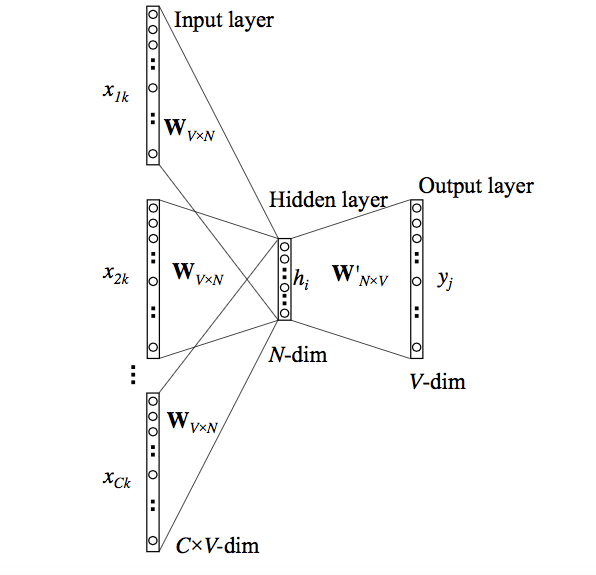
\includegraphics[width=8cm]{./images/CBOW.jpg}
  \label{fig:CBOW}
  }
  % \hspace{5pt}
    % \hspace{+5mm}
  \subfloat[skip-gram]{
  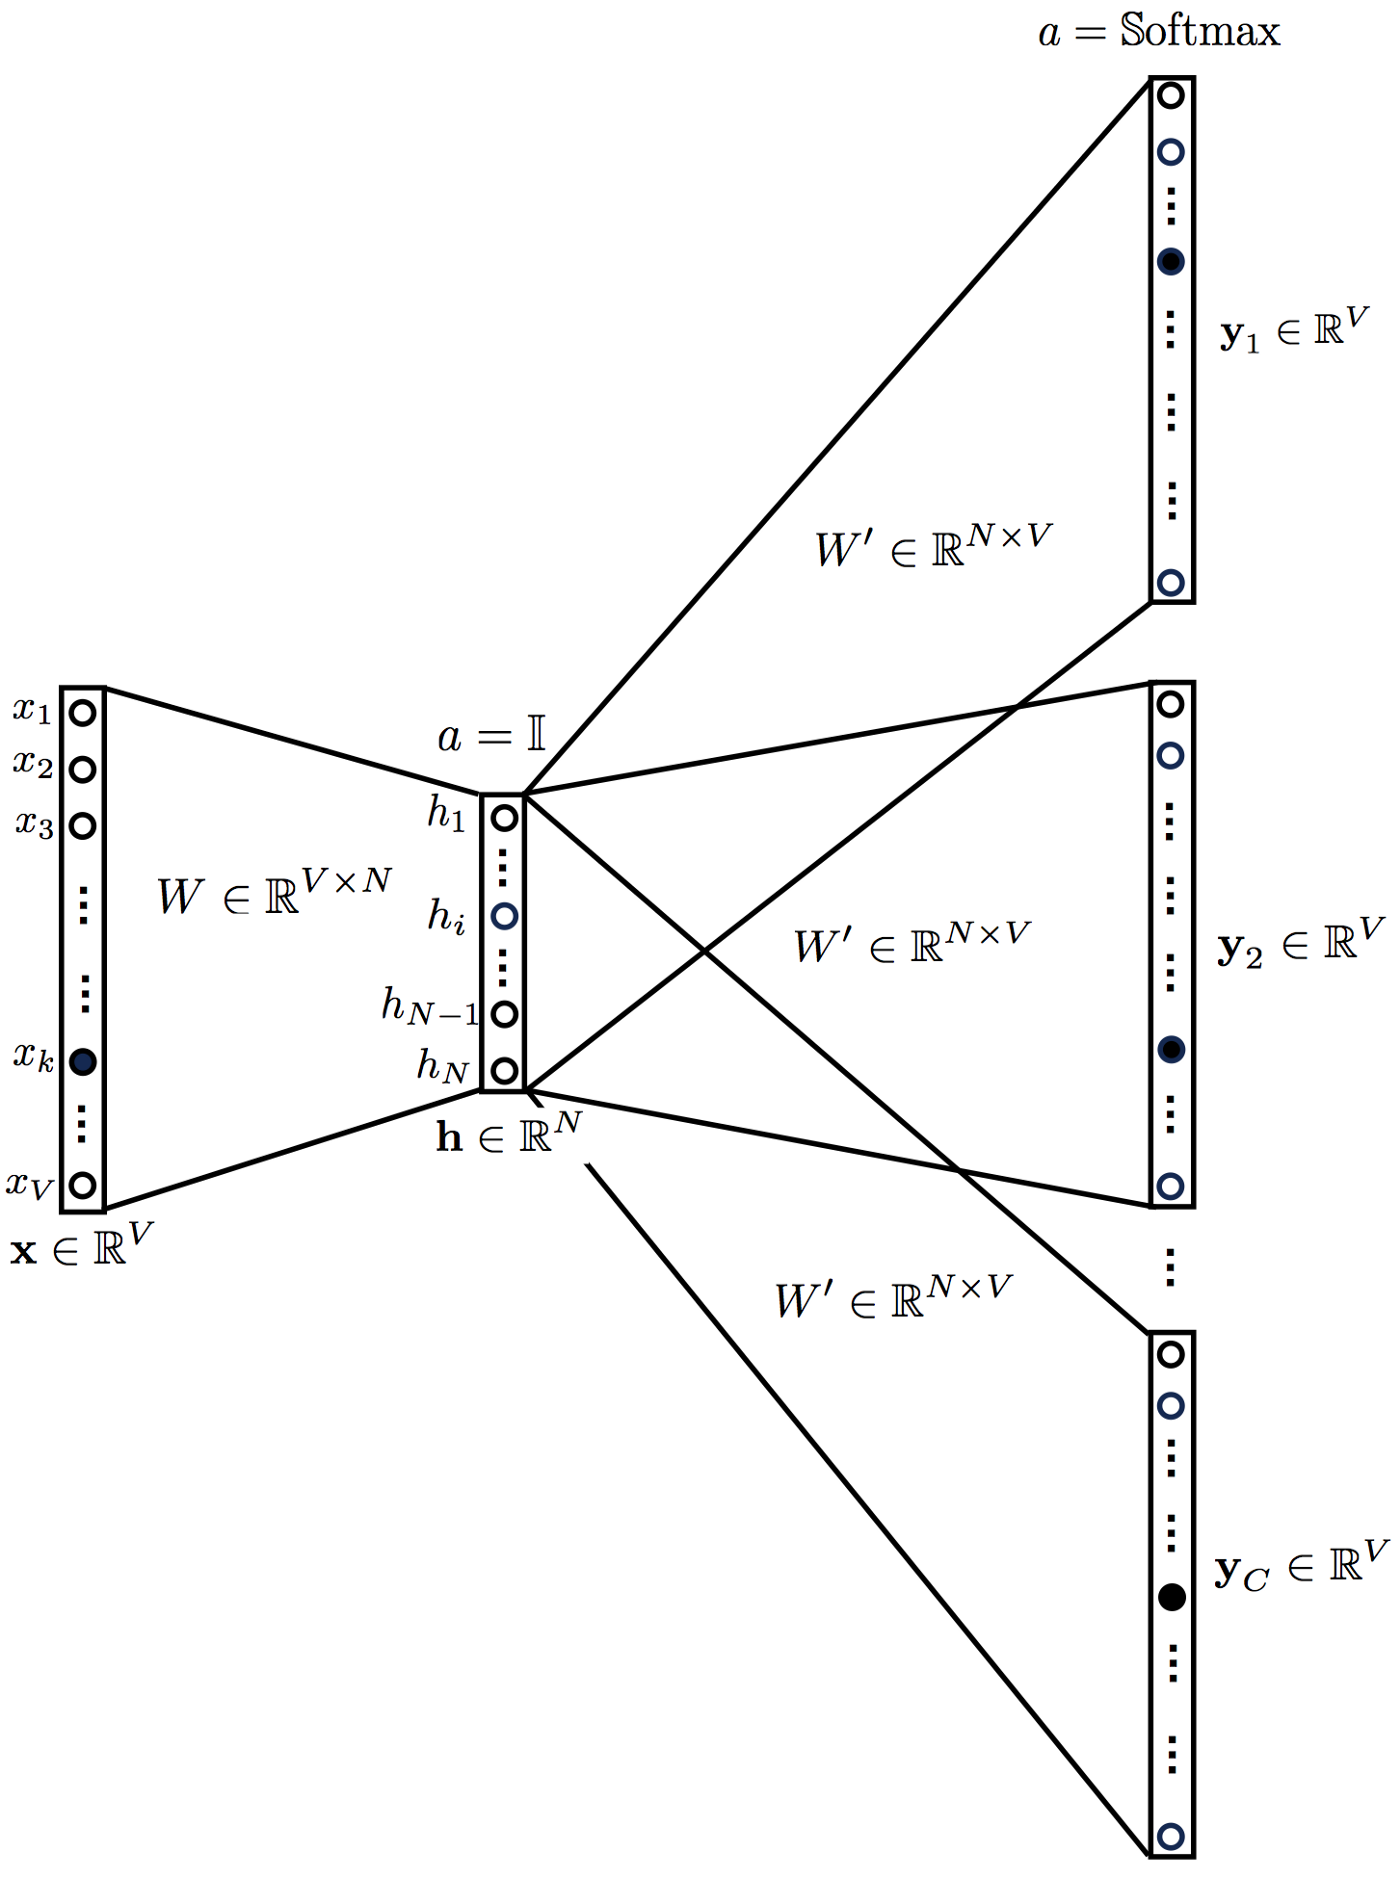
\includegraphics[width=6cm]{./images/skip.jpg}
  \label{fig:skip}
  }
  \caption{两种词向量模型\cite{mikolov2013distributed}}
  \end{figure}

\section{循环神经网络}

\subsection{RNN}

循环神经网络(RNN)是一种特殊的神经网络,其前一步的输出将作为输入输入到当前步骤。在传统的神经网络中,
所有输入和输出都是彼此独立的,但是在需要预测句子的下一个单词的情况下,需要前一个单词的信息作为支撑,
因此需要记住前一个单词。为解决此类问题,RNN诞生了,它借助“隐藏层”解决了这个问题。
RNN的最重要的功能是“隐藏状态”,它可以记住一些有关序列的信息。

RNN有一个“内存”,可以记住有关已计算内容的所有信息。在每一层的循环中,对输入使用相同的参数,
执行相同的任务以产生输出,这大大降低了参数的复杂性。
虽然其他网络在前馈过程或反向传播过程中沿线性方向“行进”,但循环网络遵循循环关系而不是前馈传递,并通过时间使用反向传播进行学习。
循环神经网络由多个固定的激活功能单元组成,每个时间步长一个功能单元。
每个单元都有一个内部状态,称为单元的隐藏状态。此隐藏状态表示过去在给定时间步长上当前网络已掌握的知识。
此隐藏状态会在每个时间步更新,以表示网络对过去的了解做出的改变变化。

\begin{figure}[htbp]
  \centering
  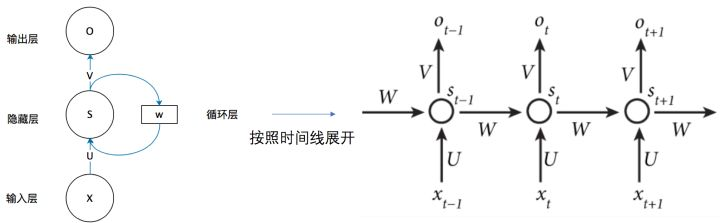
\includegraphics[scale=0.5]{./images/rnn.jpg}
  \caption{循环神经网络}
  \label{fig:rnn}
\end{figure}

上图\ref{fig:rnn}显示了将RNN展开为完整网络的过程,rnn可以被我们展开为我们想要的任意层数。例如,
如果我们输入的序列是5个单词的句子,则该网络将展开为5层神经网络,每个单词一层。对于上图具体来说,
$x_{t}$是时刻t的输入,例如,$x_{1}$ 可以是与句子的第二个单词相对应的one-hot向量。
$s_{t}$是时刻t的隐藏状态,这是网络的“记忆”,$s_{t}$根据先前的隐藏状态和当前步骤的输入来计算

\begin{equation}
  s_{t}=f(U x_{t}+W s_{t-1})
  \end{equation}

激活函数f通常是诸如tanh或ReLU之类的非线性函数,$s_{-1}$计算第一个隐藏状态所需的,通常初始化为全零。
$o_{t}$是时刻t的输出,例如,如果我们想预测句子中的下一个单词,那么它将是整个词汇表中单词的概率分布
\begin{equation}
  o_t = \mathrm softmax (V s_t)
  \end{equation}

  可以将隐藏状态$s_{t}$视为网络的记忆,$s_{t}$捕获有关先前时间步中发生的所有情况的信息。步骤t的输出$o_{t}$仅基于时间t的记忆进行计算,
  但是在实际情况中会有问题,因为$s_{t}$通常无法从太早时间之前捕获信息。与传统的深度神经网络在每一层使用不同的参数不同,
  RNN图中U,V,W在所有步骤中共享相同的参数。这是因为在每个步骤都执行相同的任务,只是输入的内容不同,这大大减少了需要学习的参数总数。
  上图在每个时间步都有输出,但是根据任务的不同,可能有些是没有必要的。例如,在预测句子的情感时,我们可能只关心最终的输出,而不关心每个单词的情感。
  同样,我们可能不需要每个时间步都输入。RNN的主要特征是其隐藏状态,该状态能够捕获有关序列的一些信息。


  
\subsection{LSTM}
  RNN的优势在于它可以将先前的信息连接到当前任务,例如使用先前的视频帧可能会有助于对当前帧的理解。
  考虑一种语言模型,该模型试图根据前一个单词预测下一个单词。
  如果试图预测“the clouds are in the sky”的最后一个词,则不需要任何进一步的上下文,很明显,下一个词将是“sky”,
  在这种情况下,如果相关信息与所需信息之间的差距很小,则RNN可以很好的学习使用过去的信息。
  但是在某些情况下,我们需要更多的上下文。考虑尝试预测文本“I grew up in France \dots I speak fluent French.”中的最后一个词,
  最临近的信息表明,下一个词可能是一种语言的名称,但是如果想缩小哪种语言的范围,需要从更远的地方来追溯“法国”的信息。相关信息与这些相关信息被需要的地方之间的差距很大是完全可能的,
不幸的是,随着差距的扩大,RNN无法处理这一问题。

长短期记忆网络(通常称为“LSTM”)是一种特殊的RNN,能够学习序列的长期依赖关系,被明确设计为能够长时间记住信息的结构,
主要解决长序列训练过程中的梯度消失和梯度爆炸问题,它是由Hochreiter&Schmidhuber(1997)提出的,
并在随后的工作中被许多人改进和推广,它在各种问题上都表现出色,现已被广泛使用。
所有的递归神经网络都具有重复模块链的形式,在标准RNN中,此重复模块将具有非常简单的结构,例如单个tanh层。
LSTM也具有这种链状结构,但是重复模块具有与传统rnn不同的结构,它不是只有一个神经网络层,而是有四个,以非常特殊的方式进行交互。

\begin{figure}[htbp]
  \centering
  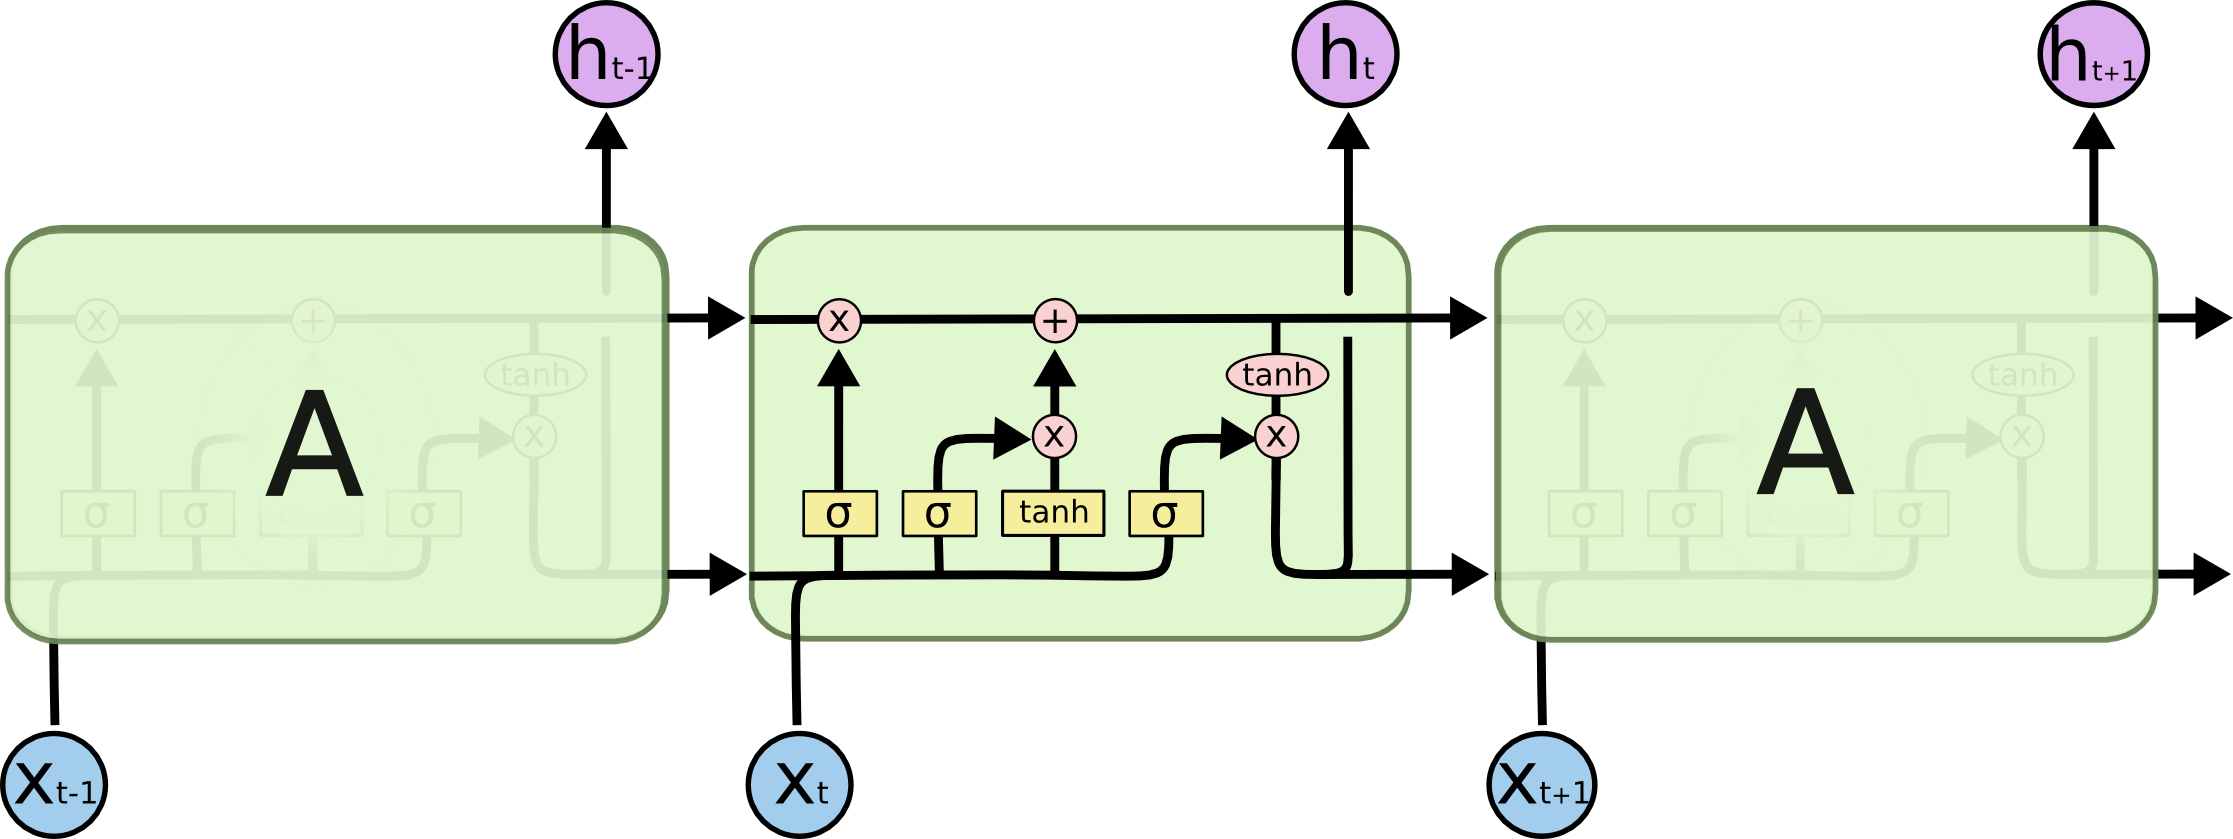
\includegraphics[scale=0.8]{./images/LSTM.jpg}
  \caption{LSTM单元模块\cite{sundermeyer2012lstm}}
  \label{fig:LSTM}
\end{figure}

LSTM结构中的关键元素是cell状态,对应图中贯穿顶部的水平线,cell像传送带一样连接起来,信息流沿整个链直线传播,只有一些较小的线性相互作用,因此信息能够非常容易地不加改变地流动。
LSTM具有删除或向单元状态添加信息的能力,这些功能由称为门的结构控制,Gates能够选择性地让信息通过,它由sigmoid神经网络层和点乘运算组成。
sigmoid输出介于0和1之间的数字,描述应允许信息流中的多少通过。值为零表示“不让任何内容通过”,而值为1表示“让所有内容通过”。
LSTM的第一步是确定要从单元状态中丢弃的信息,该决定由称为“遗忘门”的sigmoid层决定,它输入$h_{t-1}$和$x_{t}$,并对单元格$c_{t-1}$状态中的每个数字输出一个介于 0 和 1的值,
1表示“完全保留”,而0表示“完全遗忘”:
\begin{equation}
  f_{t}=σ(W_{f}\cdot[h_{t-1},x_t]+b_{f})
  \end{equation}

  下一步是确定要在cell状态下存储哪些新信息,这包括两个部分。首先,一个称为“输入门”的sigmoid层决定了我们将更新哪些值。
  接下来,tanh层创建一个新候选值的向量$\tilde{C}_{t}$,可以将其添加到状态中。之后,我们将两者结合起来以进行状态更新:
  \begin{equation}
    i_{t} =\sigma\left(W_{i} \cdot\left[h_{t-1}, x_{t}\right]+b_{i}\right) 
  \end{equation}  
    \begin{equation}
      \tilde{C}_{t} =\tanh \left(W_{C} \cdot\left[h_{t-1}, x_{t}\right]+b_{C}\right)
      \end{equation}   

然后需要更新旧单元格状态$C_{t-1}$并进入新的单元状态$C_{t}$,前面的步骤已经确定了要做什么,只需要执行即可。
将旧状态乘以 $f_{t}$,让模型忘记决定忘记的信息,然后添加$i_{t} * \tilde{C}_{t}$,这是新的候选值,
根据此决定我们更新每个状态值的大小。
\begin{equation}
C_{t}=f_{t} * C_{t-1}+i_{t} * \tilde{C}_{t}
\end{equation} 

最后需要决定要输出的内容,输出的值将基于过滤后的cell状态。
首先通过一个sigmoid层决定要输出单元状态的哪些部分,
然后通过tanh乘以sigmoid层的输出得到最终的结果,即前文提到的隐层状态$h_{t}$。
\begin{equation}
  o_{t}=\sigma\left(W_{o}\left[h_{t-1}, x_{t}\right]+b_{o}\right)
\end{equation} 
\begin{equation}
  h_{t}=o_{t} * \tanh \left(C_{t}\right)
\end{equation}


\section{注意力机制}
注意力机制是深度学习领域中最强大的理念之一,它基于一种常识性的直觉,即我们在处理大量信息时“关注”某个部分,这个简单而强大的概念彻底改变了该领域,
且不仅在自然语言处理任务上带来了许多突破,还包括推荐、医疗保健分析、图像处理和语音识别等。
许多文本信息采用序列格式,例如单词、句子和文档。Seq2Seq是一个分为两部分的深度学习架构,用于将序列输入映射到序列输出,
最初是针对机器翻译任务而提出的,但可将其应用于其他序列到序列的映射任务,例如问题检索。
但是,Seq2Seq架构的潜在问题是,某些信息可能无法通过固定长度的矢量(即编码器的最终隐藏状态)捕获。
在处理长句子时,由于梯度爆炸等原因,RNN无法将足够的信息发送到句子的末尾,因此这会成为问题。
因此,Bahdanau等\cite{bahdanau2014neural}提出注意力机制,对机器翻译这一任务,循环神经网络每一个步长输出时,都会将上下文向量和所有词汇做语义相似度的计算得到每个词汇的权值(注意力权值),
将所有词汇按权值计算加权和得到融入注意力的输入表示,这样计算的原理时翻译结果输出的词受输入的各个词汇影响不同,通过注意力权值来显示建模这种影响程度。
直观上attention机制使与解码层输出相关性的高的输入权值更高,从而使模型达到更好的性能。

self-attention是attention的变种,适用于文本分类等场景,通过计算序列中的当前词和所有其他词的相似度进而得到与当前词相关的上下文向量,
用上下文向量代替原有输入向量做后续的处理。
自我关注机制允许输入彼此交互“自我”并找出他们应该更多关注的对象,输出是这些交互作用和注意力得分的加权和。
\begin{figure}[htbp]
  \centering
  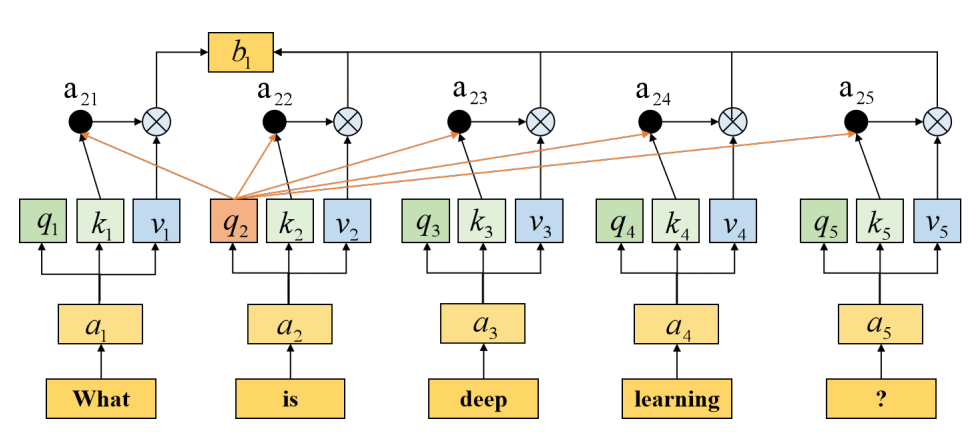
\includegraphics[width=13cm]{./images/attention.png}
  \caption{attention机制}
  \label{fig:attent}
\end{figure}

\section{transformer}
Transformer\cite{vaswani2017attention}是一种新颖的用于文本处理的架构,它使用了之前提到的注意力机制。
像RNN一样,Transformer也通过两个部分(编码器和解码器)将一个序列转换为另一个序列,
但它与先前的序列到序列模型不同,因为它并不包含任何递归神经网络网络(如GRU,LSTM等)。
在Transformer提出以前,循环网络是捕获序列中依存关系的最佳方法之一。 
但是,有研究表明,仅具有注意力机制而没有任何RNN(递归神经网络)的体系结构可以提升翻译任务的结果,
Transformer的提出者用BERT验证了这一点。

\begin{figure}[htbp]
  \centering
  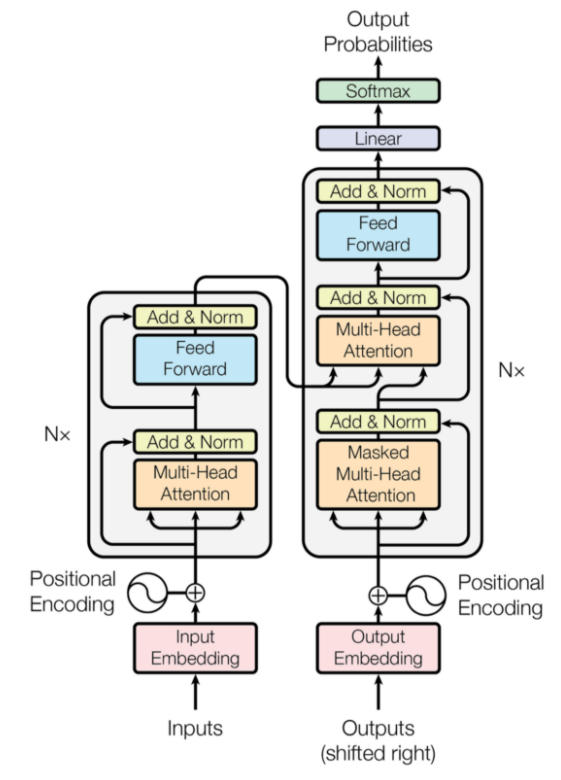
\includegraphics[width=8cm]{./images/transformer.png}
  \caption{transformer架构图\cite{vaswani2017attention}}
  \label{fig:transformer}
\end{figure}

如图\ref{fig:transformer},编码器在图中左侧,解码器在图中右侧。 
编码器和解码器均由可以相互堆叠多次的模块组成,这在图中用$N_x$描述。 
编码器和解码器均主要由多头注意力和前馈神经网络组成,输入和输出(目标语句)首先被嵌入到n维空间中,
同时该模型的一个微小但重要的改进是加入了单词的位置编码,由于Transformer没有可以记住序列位置的循环神经网络,
因此我们需要以某种方式赋予序列中的每个单词位置信息,因为顺序信息对序列文本至关重要,
这些位置将添加到每个单词的嵌入表示形式(n维向量)中。

\section{预训练模型}
NLP的最大挑战之一是缺乏足够的训练数据,从全局资源来看有大量的文本数据可用,但是如果对于创建特定任务的数据集,特别是某些领域,
最终仅能得到数千或数万有个工标记的数据。不幸的是,为了表现良好,基于深度学习的NLP模型需要大量的数据,在数百万或数亿的带标注的训练样本上进行训练时,
模型效果相比少数据量会有质的提升。为了帮助弥合数据鸿沟,研究人员开发了多种技术,可在网络上使用大量无标注的文本数据来训练通用语言表示模型(称为预训练),
然后,可以在特定任务的较小数据集上微调这些通用的预训练模型。例如,在处理诸如问答系统和情感分析之类的问题时。与从头开始对较小的特定任务的数据集进行训练相比,
预训练模型方法可显着提高准确性。BERT\cite{devlin2018bert}是这些技术中用于NLP预训练的最新应用,在深度学习社区引起了轰动,因为它在各种NLP任务中都达到了最优异的成果。

预训练模型语言建模的任务是根据上下文“填补空白”,例如,给定
“The woman went to the store and bought a( )of shoes”,模型可能会判定“cart”一词在20%的情况合适,而“pair”一词在80%的情况合适。
在BERT之前,语言模型会在训练期间从左到右或从左到右和从右到左组合查看文本序列。这种单向方法很适合生成句子,即预测下一个单词,
将其附加到序列中,然后预测再下一个单词,直到获得完整的句子。
BERT并没有预测序列中的下一个单词,而是使用了一种称为Masked LM(MLM)的新颖技术:它随机屏蔽句子中的单词,然后尝试预测它们。
掩蔽意味着该模型是无方向性,并且它使用句子的整个上下文来预测被掩盖的单词。与以前的语言模型不同。

% 预训练的语言表示可以是上下文无关或上下文相关的,上下文相关的模型又可以分为单向和双向的。
% word2vec之类的上下文无关模型会为词汇表中的每个单词生成唯一的单词嵌入表示。
% 例如,单词“bank”在“bank account”和“bank of the river”中将具有相同的向量表示。
% 另一方面,基于上下文的模型会基于句子中的其他单词生成每个单词的表示形式。例如,在句子“I accessed the bank account”,
% 单向上下文模型将基于“I accessed the”而不是“account”来表示“bank”。但是,BERT从前部和后部上下文信息(“I accessed the … account”)表示“bank”,
% 它从深度神经网络的最底层开始,使其深度双向化。

BERT依赖于Transformer,一个基本的Transformer由一个读取文本输入的编码器和一个对任务进行预测的解码器组成。
BERT编码器的输入是一系列token,这些token首先被转换为矢量,然后在神经网络中进行处理。
但是在开始处理之前,BERT需要对输入进行处理并用一些额外的元数据修饰:

1.令牌嵌入:在第一个句子的开头将[CLS]令牌添加到输入的单词令牌中,并在每个句子的末尾插入[SEP]令牌。

2.段嵌入:将指示输入属于句子A或句子B的标记添加到每个标记,这使编码器能够区分输入属于哪个句子。

3.位置嵌入:将位置嵌入添加到每个标记,以指示词在句子中的位置。
\begin{figure}[htbp]
  \centering
  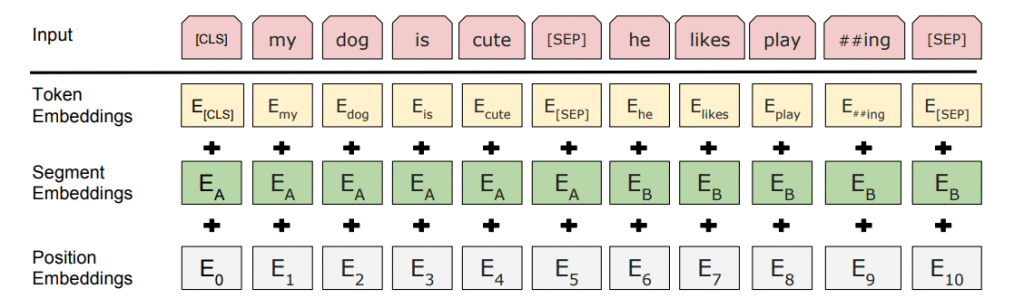
\includegraphics[scale=0.5]{./images/inputBert.jpg}
  \caption{bert的输入处理\cite{devlin2018bert}}
  \label{fig:inputBert}
\end{figure}

BERT不会尝试预测句子中的下一个单词,训练时使用以下两种策略:

Masked LM (MLM),
随机掩盖输入中15%的单词(用[MASK]令牌代替),将处理好的序列输入模型,然后根据序列中其他未屏蔽单词提供的上下文信息预测被屏蔽的词,
但是,这种掩盖方法存在一个问题,模型只会预测输入中存在的词,而我们希望模型尝试预测正确的token,而不管该token是否存在于输入中。
要解决此问题,bert在训练时,对于被选中要被屏蔽的词,有80%按原方案被替换为令牌[MASK],10%被替换为随机token,剩下10%保持不变。

Next Sentence Prediction,
为了理解两个句子之间的关系,BERT训练过程还进行了下一个句子预测,具有这种理解的预训练模型可以解决诸如回答问题之类的任务。
在训练过程中,该模型将句子对作为输入,并学习预测第二个句子是否是原始文本中的下一个句子。第二句出现在第一句之后的概率有50%,剩下50%出现的是语料库中随机的句子。
为了预测第二句话是否与第一句话相连,整个输入序列都会经过基于Transformer的模型,使用简单的分类层将[CLS]token的输出转换为2×1形状的向量,
并使用softmax来决策。

\section{本章小结}